% Adjust these for the path of the theme and its graphics, relative to this file
%\usepackage{beamerthemeFalmouthGamesAcademy}
\usepackage{../../beamerthemeFalmouthGamesAcademy}
\usepackage{multimedia}
\graphicspath{ {../../} }

% Default language for code listings
\lstset{language=C++,
        morekeywords={each,in,nullptr}
}

% For strikethrough effect
\usepackage[normalem]{ulem}
\usepackage{wasysym}
\usepackage{gensymb}
\usepackage{pdfpages}

% http://www.texample.net/tikz/examples/state-machine/
\usetikzlibrary{arrows,automata}

\newcommand{\modulecode}{COMP260}\newcommand{\moduletitle}{Distributed Systems}\newcommand{\sessionnumber}{5}

\begin{document}
\title{\sessionnumber: }
\subtitle{\modulecode: \moduletitle }

\frame{\titlepage} 
\begin{frame}
	\begin{figure}
		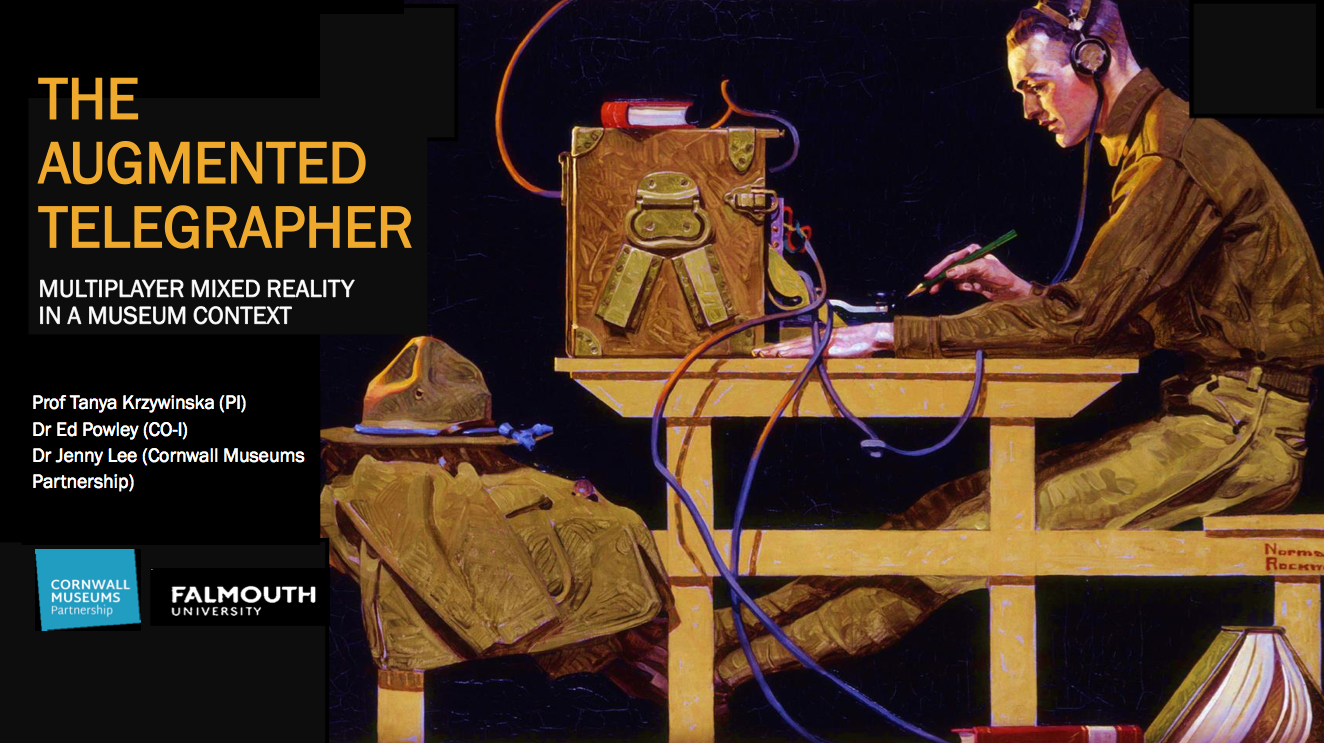
\includegraphics[scale=0.2]{assets/tel.png}
		
	\end{figure}
	alcwyn.parker@falmouth.ac.uk
\end{frame}

% LEARNING OUTCOMES
\begin{frame}
	\frametitle{Virtual and Augmented Reality Overview:}
	
	\textbf{Learning Outcomes:}
	
	\begin{itemize}
		\item \textbf{Explain} the difference between augmented \& virtual reality. 
		\item \textbf{Discuss} the differences between immersion and presence
		\item \textbf{Outline} the various technologies and human factors that combine to create a sense of presence in the user
	\end{itemize}
	
	\textbf{3 Weeks distilled into one hour}

\end{frame}

\begin{frame}
	\frametitle{A Word of Warning}
	AR/VR are both emerging technologies and thus, they borrow language from other similar disciplines such as \textbf{photography}, game development, film studies and 3D design. This appropriation of lexicons can be confusing and there will be some overlap in relation to key terms and definitions.
\end{frame}

\begin{frame}
	\begin{figure}
		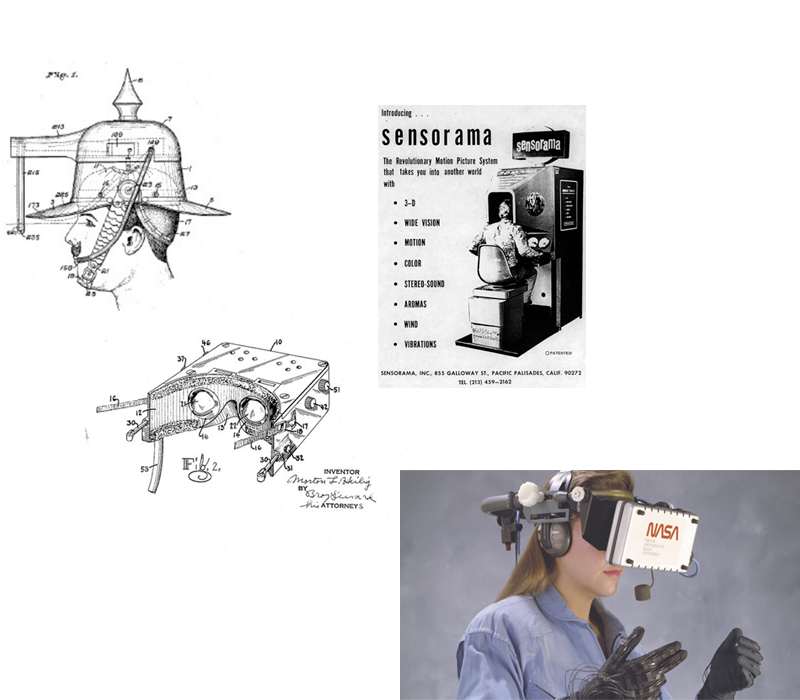
\includegraphics[scale=.6]{assets/history.png}
		\caption{\tiny{Left to Right - Pratt's head-mounted targeting interface, Heilig's Stereoscope TV Apparatus \& Sensorama, NASA's VIEW System} }
	\end{figure}
\end{frame}


\begin{frame}
	\frametitle{Forms of Reality}
	\begin{figure}
		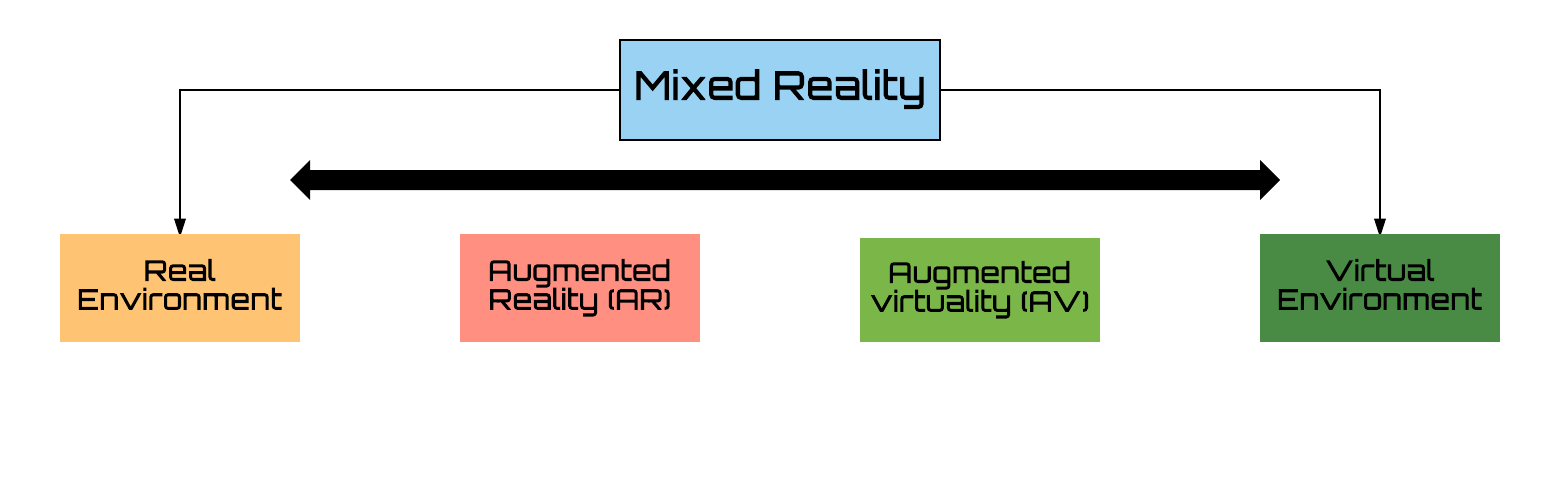
\includegraphics[scale=.2]{assets/continuum.png}
		\caption{The Virtuality Continuum - Milgram \& Kishino}
	\end{figure}
\end{frame}


\begin{frame}
	\begin{figure}
		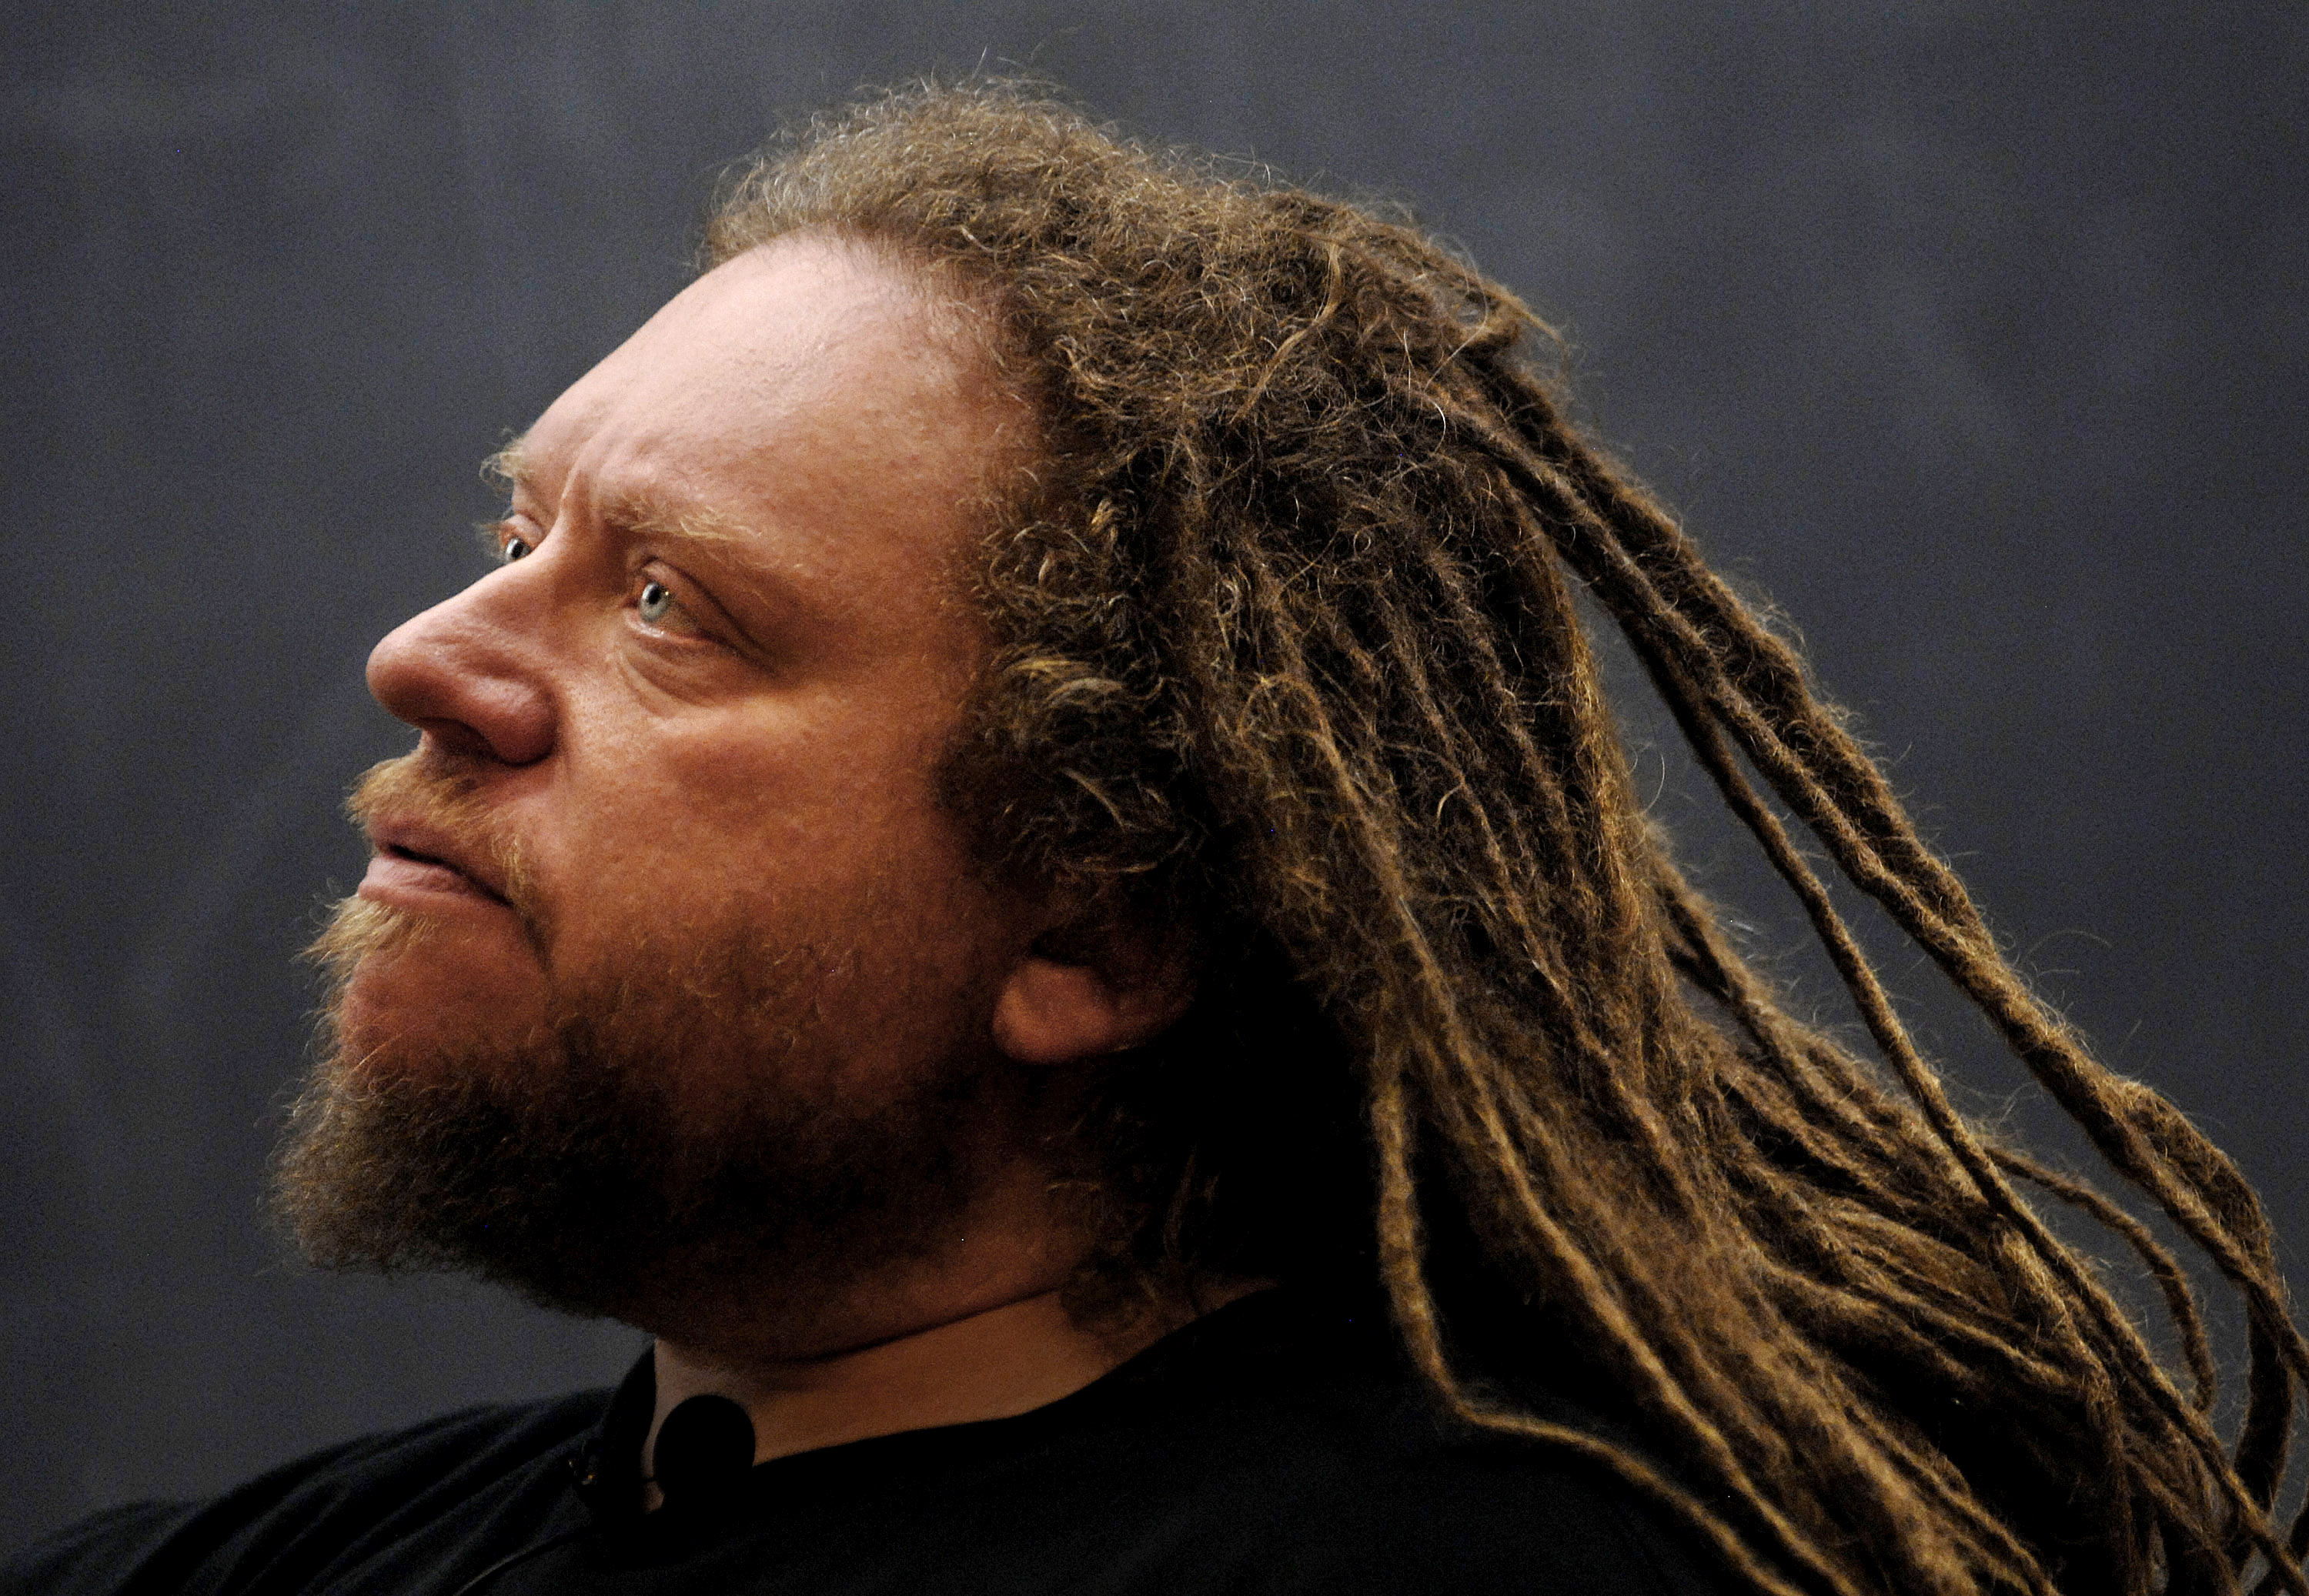
\includegraphics[scale=0.3]{assets/lanier.jpg}
	\end{figure}
	The term `virtual reality' was coined by Jaron Lanier in 1987 during a period of intense research activity into this form of technology.
	
\end{frame}

\begin{frame}
	``As babies, each of us has an astonishing liquid infinity of imagination on the inside; that butts up against the stark reality of the physical world. That the baby's imagination cannot be realised is a fundamental indignity that we only learn to live with when we decide to call ourselves adults. With virtual reality you have a world with many of the qualities of the physical world, but it doesn't resist us. It release us from the taboo against infinite possibilities. That's the reason virtual reality electrifies people so much.''

\end{frame}


% Hands up who has had a go with....
% run through some of the introduction from book.

%REALITY SYSTEMS
\begin{frame}
	\frametitle{Reality Systems - Hardware}
	
	\begin{columns}
		
		\begin{column}{0.5\textwidth}
			\textbf{Display Types:}
			\begin{itemize}
				\item Head-Mounted Displays
				\item World-Fixed Displays
				\item Hand-held Displays (tablets = floating, mobile = personal)
			\end{itemize}
		\end{column}
		
		\begin{column}{0.5\textwidth}

			\textbf{Audio:}
			Spatialised Audio is preferred
			\begin{itemize}
				\item Headphones - more immersive.
				\item surround sound speakers.
			\end{itemize}
			
		\end{column}
		
	\end{columns}
\end{frame}

\begin{frame}
	\frametitle{Head-Mounted Displays (HMD)}
	\begin{figure}
		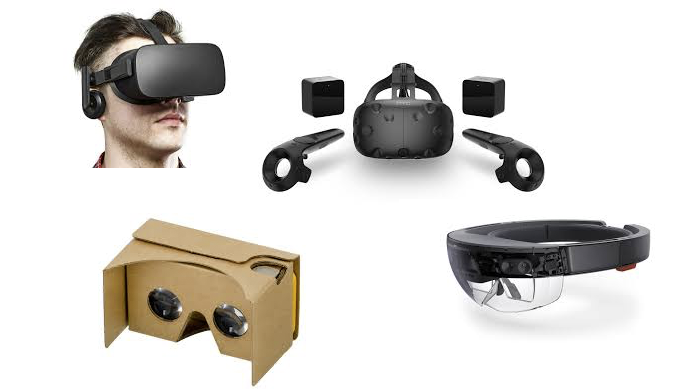
\includegraphics[scale=0.4]{assets/hmd.png}
	\end{figure}
\end{frame}


\begin{frame}
	\frametitle{And then there is Magic Leap}
	\begin{figure}
		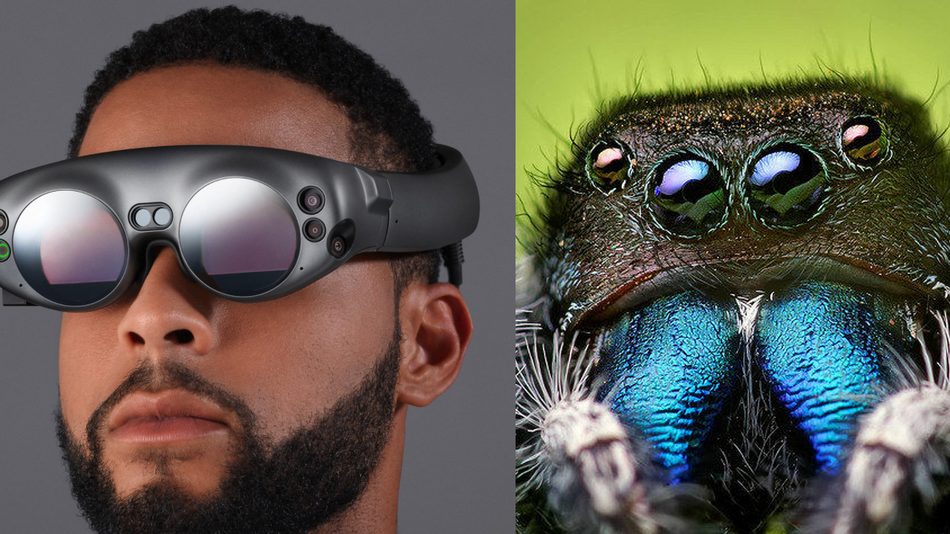
\includegraphics[scale=0.3]{assets/leap.png}
	\end{figure}
\end{frame}

\begin{frame}
	\frametitle{World-Fixed Display}
	\begin{figure}
		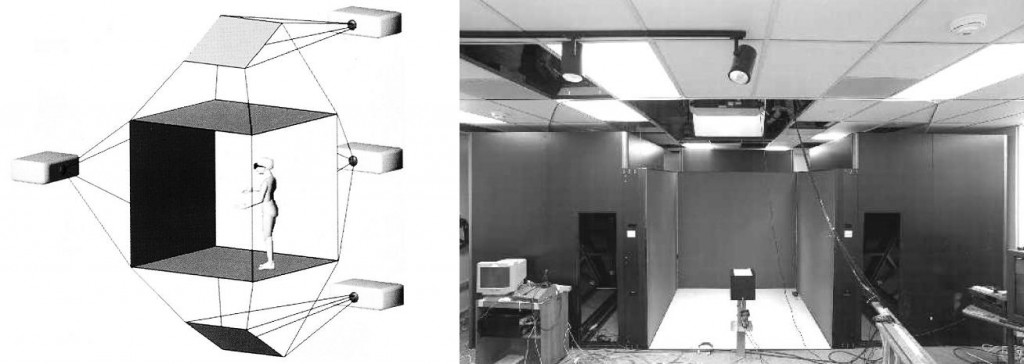
\includegraphics[scale=0.3]{assets/cave.jpg}
		\caption{Cave VR environment: A lifelike visual display is created by projectors positioned outside the CAVE and controlled by physical movements from a user inside the CAVE.}
	\end{figure}
\end{frame}

\begin{frame}
	\frametitle{Hand-held displays}
	\begin{figure}
		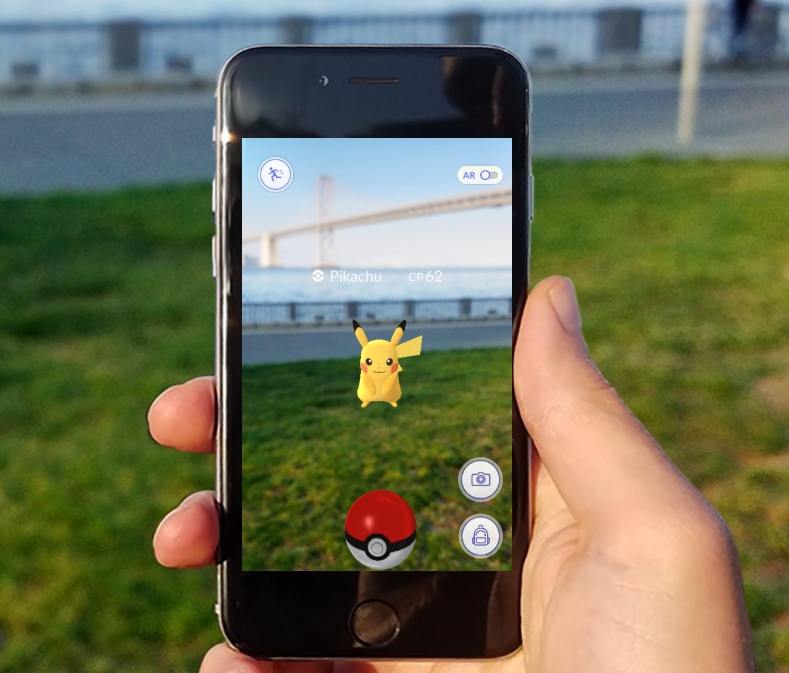
\includegraphics[scale=0.25]{assets/pgo.png}
		\caption{Pokemon Go}
	\end{figure}
	
\end{frame}

%TRACKING
\begin{frame}
	\frametitle{Tracking}
	\begin{itemize}
		\item Accelerator \& Gyro embedded in displays
		\item Leap motion - Hand Tracking
		\item Eye Tribe (Foveated rendering)
		\item Fiducials Markers
		\item Kinect2 - Skeleton Tracking
		\item Valve's Lighthouse Tracking Sensors
		\item Vive Trackers \href{https://www.youtube.com/watch?v=rJKO2WGSP_I}{(Link)}
	\end{itemize}
\end{frame}

% OUTSIDE VS INSIDE
\begin{frame}
	\frametitle{Tracking}
	\begin{figure}
		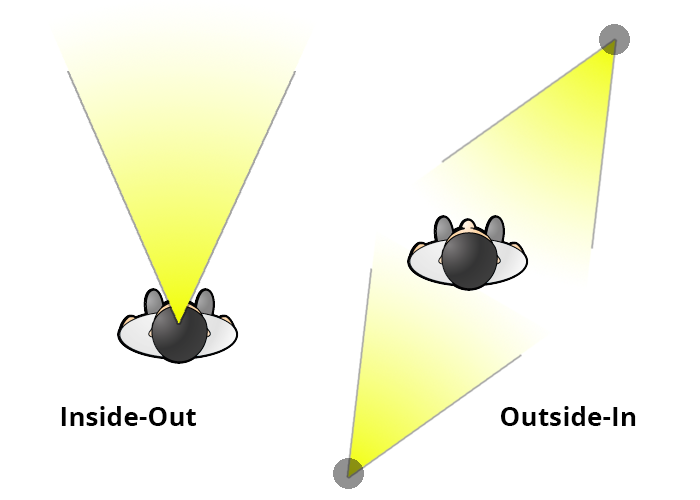
\includegraphics[scale=0.25]{assets/tracking.png}
		\caption{Pokemon Go}
	\end{figure}
\end{frame}



\begin{frame}
	\frametitle{Haptics}
	Haptics are the artificial forces between virtual objects and the user.
	\vspace{.2in}
	
	\textbf{Passive -}
	real-world physical objects that match the shapes of a virtual objects. (Doors, ledges, pillars... )
	\vspace{.2in}
	
	\textbf{Active -} Haptics can be dynamically controlled by the computer to provide a feeling of a wide range of simulated virtual objects.
	
\end{frame}

\begin{frame}
	\begin{figure}
		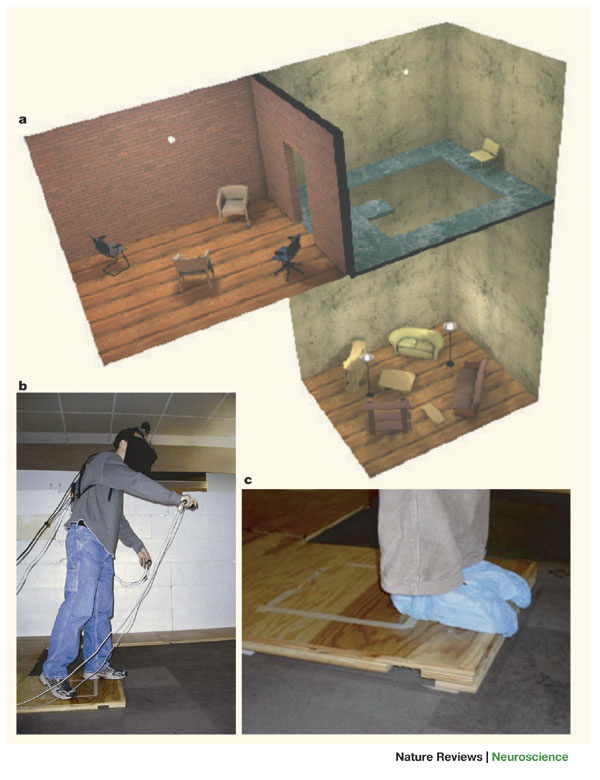
\includegraphics[scale=0.25]{assets/thepit.png}
		\caption{University of North Carolina - Pit Experiment}
	\end{figure}
\end{frame}

\begin{frame}
	
	\frametitle{Tactile Haptics}
	
	\begin{itemize}
		\item Vibrotactile - vibration passed directly or indirectly to the skin
		\item Electrotactile - electrodes passing current through the skin
		\item Proprioceptive force - provides a sense of limb movement and muscular resistance
	\end{itemize}	
	
\end{frame}

\begin{frame}
	\frametitle{Self-Grounded vs. World-Grounded Haptics}
	\begin{figure}
		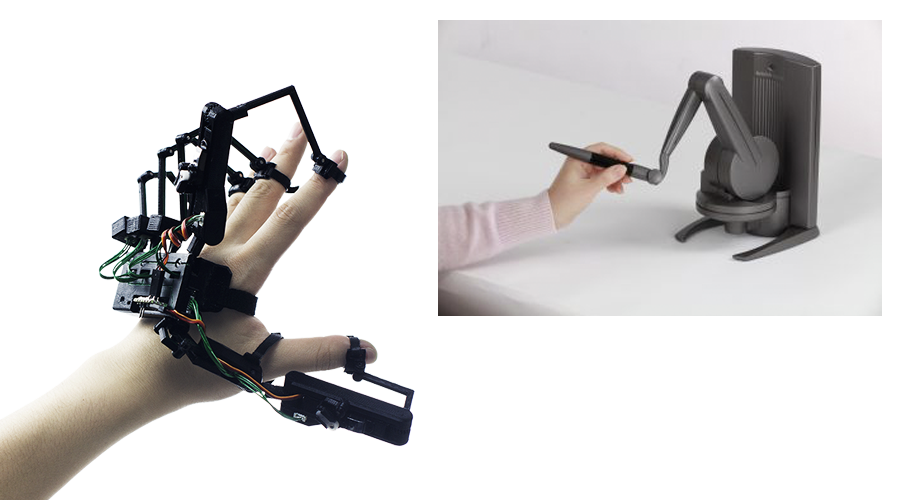
\includegraphics[scale=0.3]{assets/self-world.png}
		\caption{DexmoF2 \& Sensable's Phantom Haptic System}
	\end{figure}
	
\end{frame}

\begin{frame}
	\frametitle{Motion Platforms}
	A motion platform is a hardware device that moves the entire body resulting in a sense of physical motion and gravity. 
	\vspace{.2in}
	
	
	These systems can convey a sense of orientation, vibration, acceleration and jerking.	
	\vspace{.2in}
	
	
	[Examples]
	
\end{frame}

{
      \begin{frame}[plain]
        \begin{tikzpicture}[remember picture,overlay]
            \node[at=(current page.center)] {
                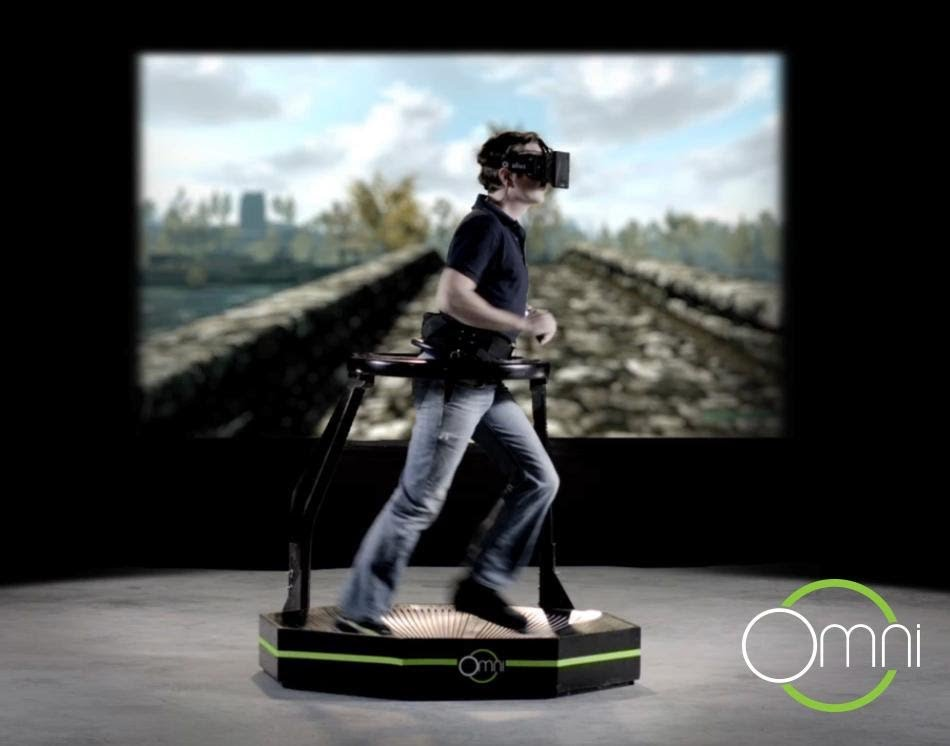
\includegraphics[width=\paperwidth]{assets/virtuix}
            };
        \end{tikzpicture}
     \end{frame}
}

{
      \begin{frame}[plain]
        \begin{tikzpicture}[remember picture,overlay]
            \node[at=(current page.center)] {
                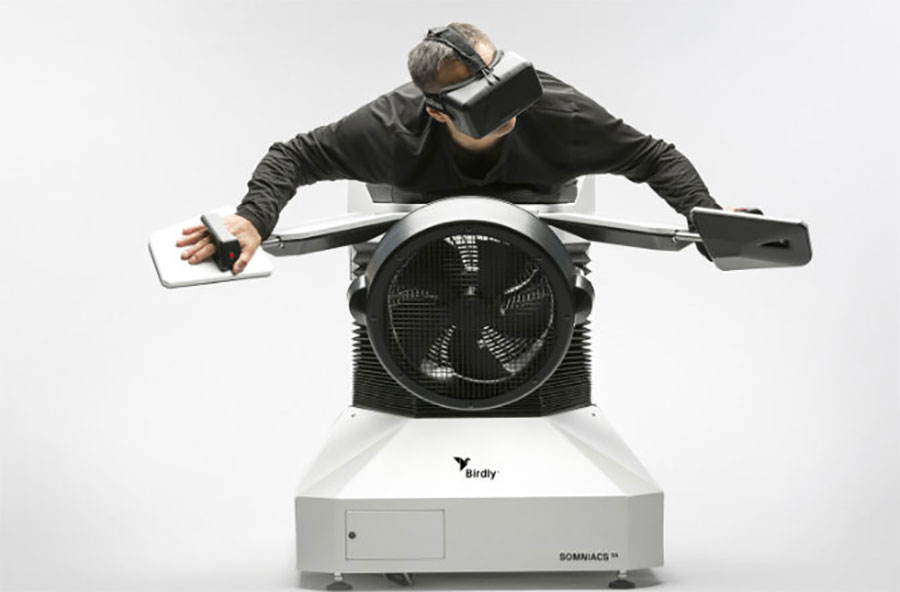
\includegraphics[width=\paperwidth]{assets/birdy}
            };
        \end{tikzpicture}
     \end{frame}
}

\begin{frame}
	\frametitle{Human-Centred Design:}
	Some tips when designing for AR \& VR
\end{frame}


% CONTINUOUS DISCOVERY 
\begin{frame}
	\frametitle{Continuous Discovery}
	Continuous discovery is the on-going process of engaging users during the design and development process. 
	\begin{itemize}
		\item \pause You can never know everything in advance of a project.
		\item \pause Waiting until the end of a build to find out that something doesn't work is unsustainable. 
		\item \pause Change is inevitable.
		\item \pause Failures are an inevitable outcome of creativity and innovation. 
	\end{itemize}
\end{frame}	

% ITERATION CYCLE
\begin{frame}
	\frametitle{Iteration}
	\begin{figure}
		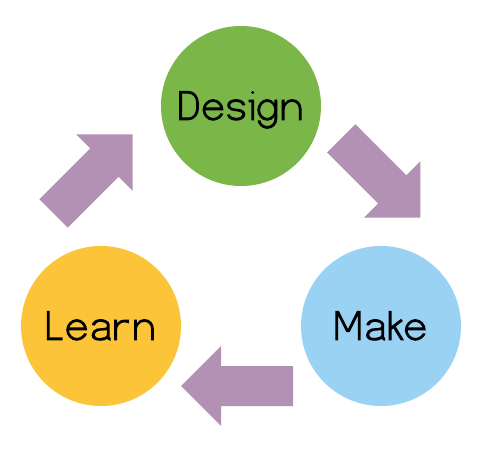
\includegraphics[scale=0.4]{assets/iteration.png}
		\caption{The Iteration Cycle}
	\end{figure}
\end{frame}

\begin{frame}
	\frametitle{\textbf{ASK QUESTIONS}}
	\begin{itemize}
		\item Feedback is crucial - you require a lot of trust from the user! 
		\item Ask lots of questions.
		\item Do not trust assumptions. 
		\item Common misconception.
	\end{itemize}
\end{frame}


\begin{frame}
	\frametitle{Immersion}
	Immersion is the objective degree to which a VR system and application projects stimuli onto the sensory receptors. We discuss immersion in terms of:

	\begin{itemize}
		\item Extensiveness - Range of sensory modalities targeted 
		\item Matching - Stimuli vs reality
		\item Surrounding - Extent of environment (panoramic) and tracking
		\item Vividness - The quality of simulation
		\item Intractability - The quality of the input and outputs
		\item Plot - How compelling the narrative is
	\end{itemize}
\end{frame}

\begin{frame}
	\begin{figure}
		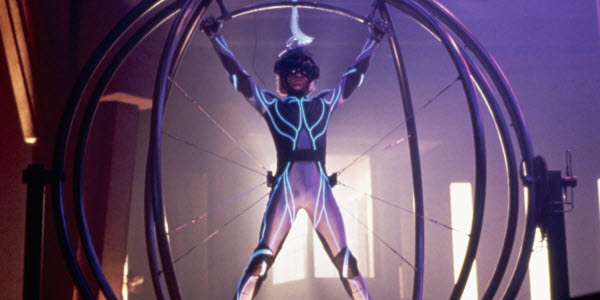
\includegraphics[scale=.6]{assets/mower} 
		\caption{The Lawnmower Man - 1992}
	\end{figure}
	Not the last Lawnmower Man ref you will see today ;)
\end{frame}


\begin{frame}
	\frametitle{Immersion vs. Presence}
	
	`Presence is the psychological state of subjective perception in which even though part or all of an individual's current experience is generated by and/or filtered through human-made technology, part or all of the individual's perception fails to accurately acknowledge the role of the technology in the experience.' \\~\\
	
	International Society for Presence Research, 2000
	\\~\\
	\href{http://ispr.info}{[ISPR Website]}	
	
\end{frame}

\begin{frame}
	\frametitle{Perceptual Modalities}
	
	``A perceptual modality can be defined as the means through which information is extracted from the environment'' (James and Galbraith, 1985) \\~\\
	
	Immersion is created by surrounding the user of the VR system in images, sound or other stimuli that provide an engrossing total environment. \\~\\
	In order to achieve an illusion of immersion a reality system must consider the perceptual modalities: \textbf{Sight}, \textbf{hearing}, touch, proprioception, \textbf{balance/motion}, smell and taste. \\~\\
	
\end{frame}

\begin{frame}
	\frametitle{Field of View and Field of Regard}
	%The \textbf{field of view} is the angular measure of what can be seen at a single point in time. 
	\begin{figure}
		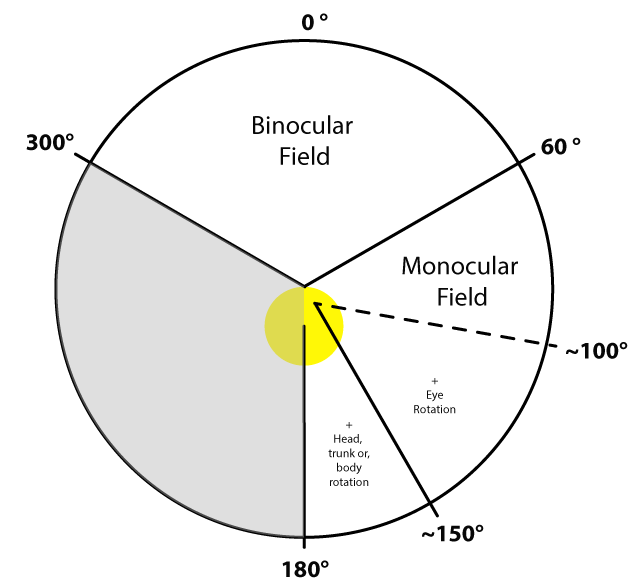
\includegraphics[scale=.3]{assets/fov} 
		\caption{Horizontal field of view of the right eye with straight ahead fixation (looking towards the top of the diagram)}
	\end{figure}
\end{frame}


\begin{frame}
	\frametitle{Chromatic Aberration }
	
	\begin{figure}
		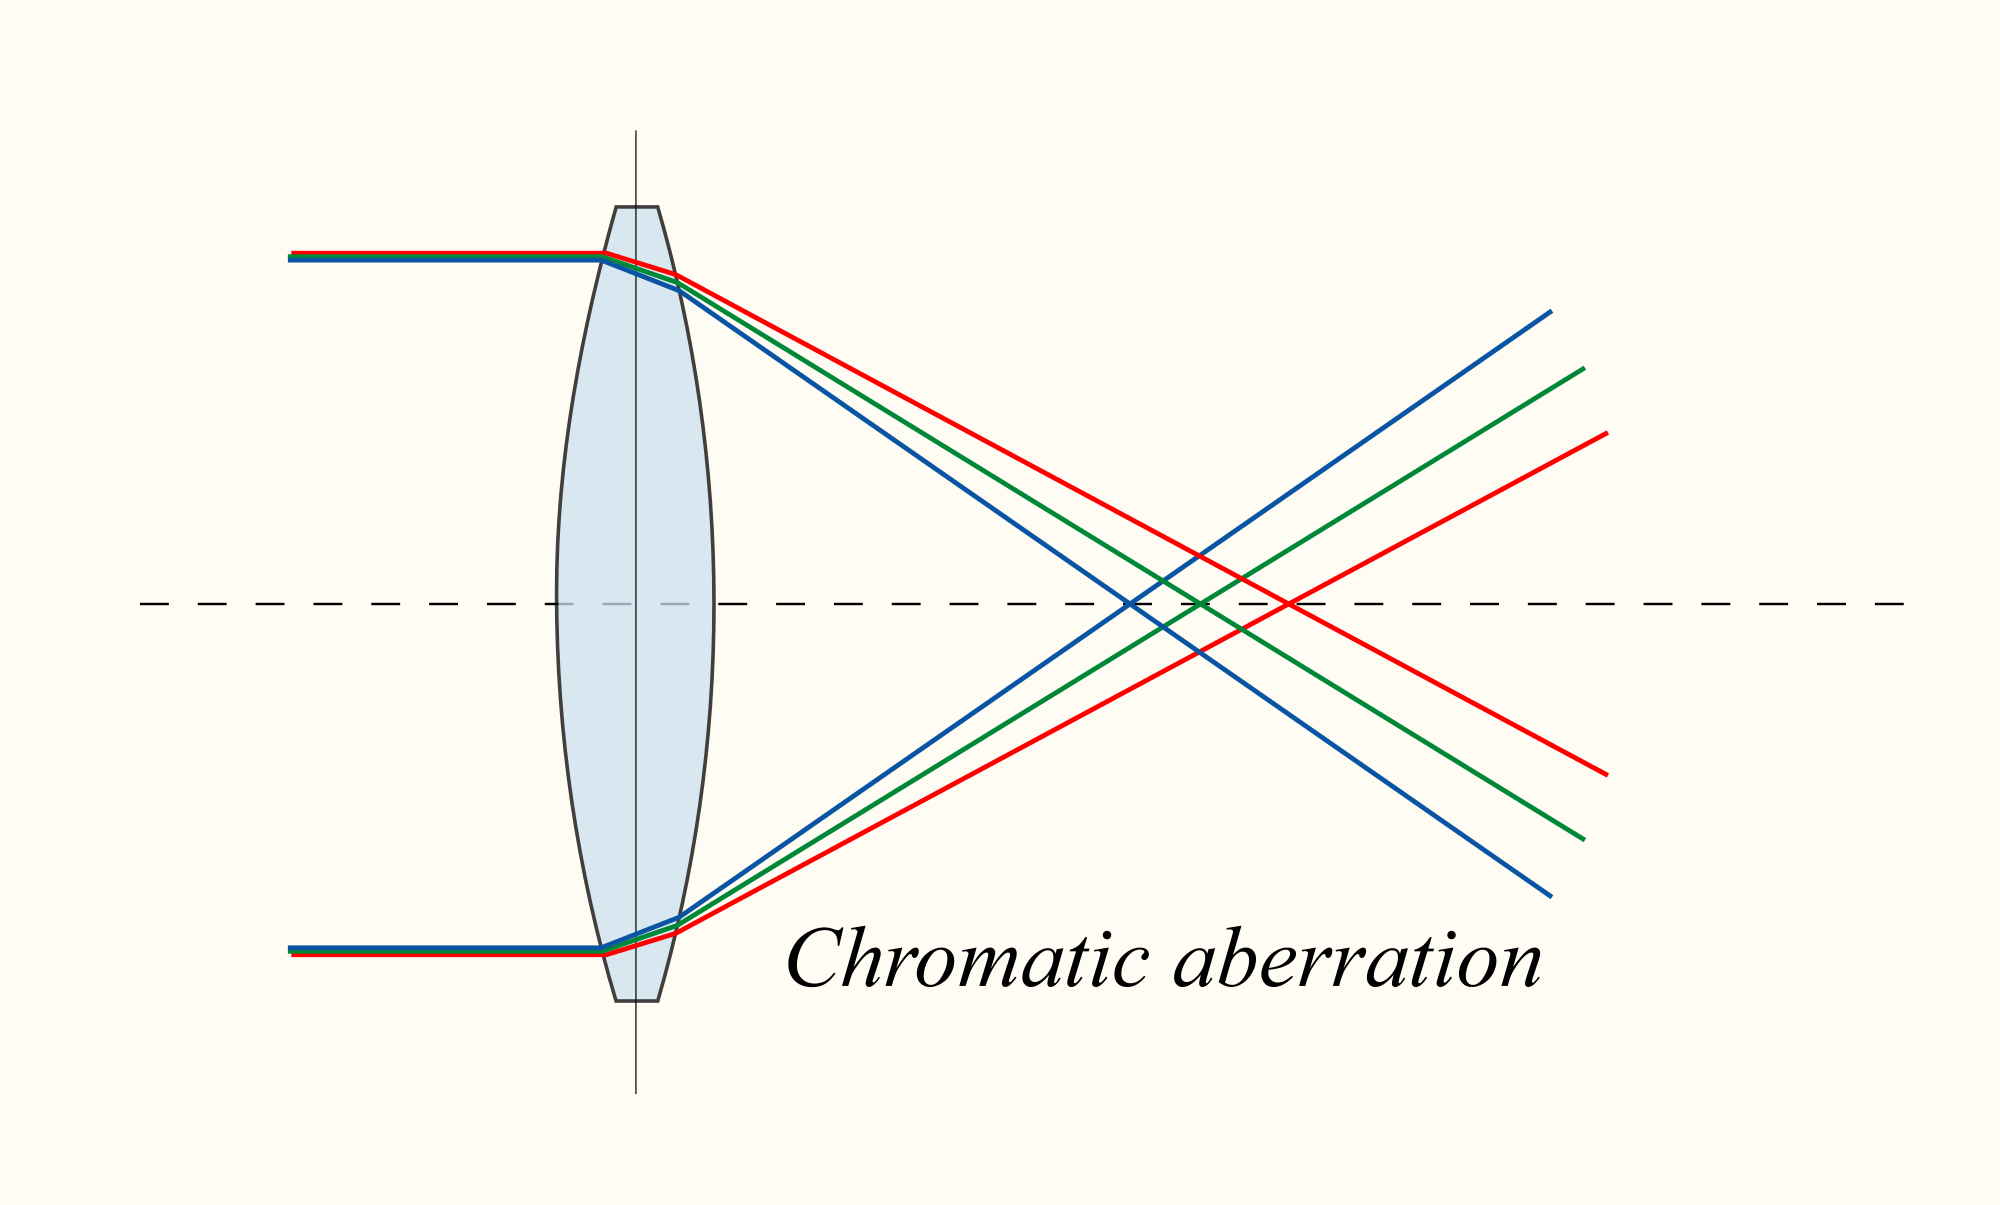
\includegraphics[scale=.1]{assets/aberration} 
		\caption{When different wavelengths of light refract at different angles. Movement of the eye can amplify the aberration. \tiny{aberration:a departure from what is normal}}
	\end{figure}
\end{frame}

\begin{frame}
	\frametitle{Vergence-Accommodation Conflict}
	
	\textbf{Vergence} - How your eyes track an object coming towards you. \\~\\

	\textbf{Accommodation} - When you pupils adjust to the objects light field. \\~\\
	
	The two actions are hardwired to work in sync as they are both trying aid the same process of tracking an object. They can be decoupled but it is not a comfortable experience for the user.

\end{frame}

\begin{frame}
	`After long session, I still have an hangover time though, as if I was on drugs the whole time and I need to readjust to reality.' \\~\\
	
	\href{https://www.reddit.com/r/oculus/comments/2clksh/question_for_dk2_owners_how_long_can_you_wear_it/cjgo683}{[link to further discussion]} \\~\\
	\href{https://www.reddit.com/r/oculus/comments/2epu1h/my_body_has_developed_a_fear_of_vr/}{and more}
	
\end{frame}

\begin{frame}
	\begin{figure}
		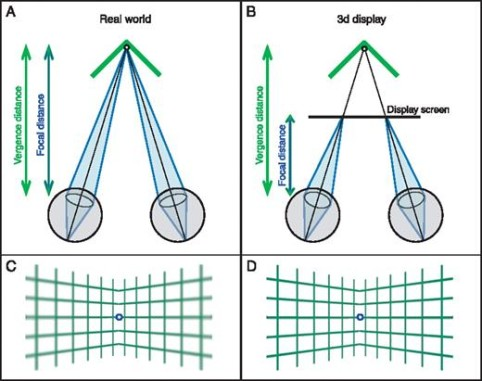
\includegraphics[scale=.7]{assets/verg} 
		\caption{Vergence-Accommodation Conflict}
	\end{figure}

\end{frame}

\begin{frame}
	\frametitle{Motion to Photon Latency}
	\begin{itemize}
		\item \textbf{Motion} - refers to the users movements in the physical space.
		\item \textbf{Photons} - The photons emitted from the HMD that are absorbed by photoreceptors (cones \& rods) on the retina.
		\item \textbf{Latency} - delay between the two. 
	\end{itemize}
	
		Put simply, motion to photon latency is the time it takes for the users movements in physical space to be visualised on the head-mounted display(HMD).
	
\end{frame}

\begin{frame}
	\frametitle{Side Effects}
	The \textless20ms motion-to-photon latency gold standard. \\~\\
	
	When the motion to photon latency is greater than 20ms or anytime there is inconsistent stimuli between the players physical body motions and the visuals displayed in the head-mounted display (HMD) then there is a good chance that motion sickness/simulator sickness will occur. \\~\\

	According to the Oculus Rift docs, other factors that can contribute to simulator sickness are:

\end{frame}

\begin{frame}
		
	\begin{itemize}
		\item Acceleration - minimize the size and frequency of accelerations
		\item Degree of control - don't take control away from the user
		\item Duration of simulator use - allow and encourage users to take breaks
		\item Altitude - avoid filling the field of view with the ground
		\item Binocular disparity - some find viewing stereoscopic images uncomfortable
		\item Field-of-View - reducing the amount of visual field covered by the virtual environment may also reduce comfort
		\item ... (the list goes on)
	\end{itemize}
	
\end{frame}

\begin{frame}
	\begin{itemize}
		\item Latency - minimize it; lags/dropped frames are uncomfortable in VR
		\item Distortion correction - use Oculus VR?s distortion shaders
		\item Flicker - do not display flashing images or fine repeating textures
		\item Experience - experience with VR makes you resistant to simulator sickness (which makes developers inappropriate test subjects)
	\end{itemize}
\end{frame}

\begin{frame}

	\begin{center}
		\frametitle{Oculus Rift Health \& Safety Guide}
		\href{https://static.oculus.com/documents/310-30023-01_Rift_HealthSafety_English.pdf}{ 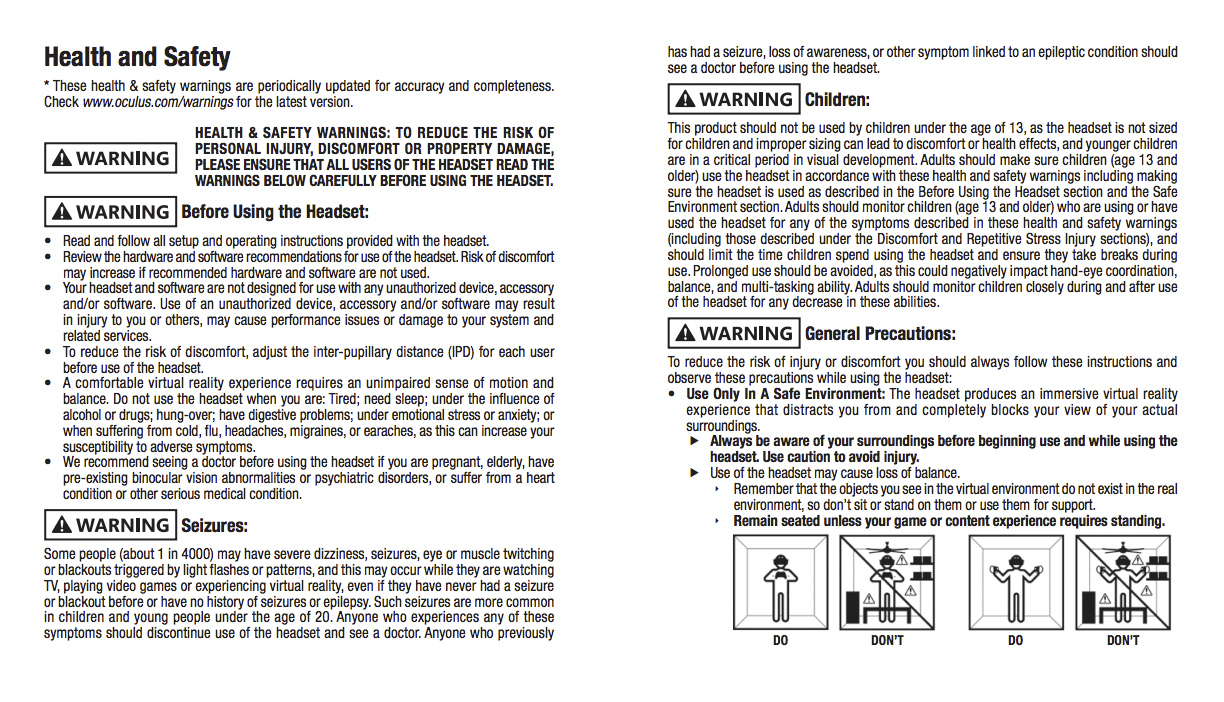
\includegraphics[scale=.45]{assets/sideeffects}  }
	\end{center}

\end{frame}

\begin{frame}
	\frametitle{Balance}
	There are three systems at work to aid in balance:
	
	\begin{itemize}
		\item Vestibular System (motion, equilibrium, spatial orientation)
		\item Proprioception (position, motion, and equilibrium)
		\item Vision (sight)
	\end{itemize}
			
\end{frame}

\begin{frame}
	\frametitle{Vestibular System}
	\begin{center}
		\href{https://www.youtube.com/watch?v=P3aYqxGesqs}{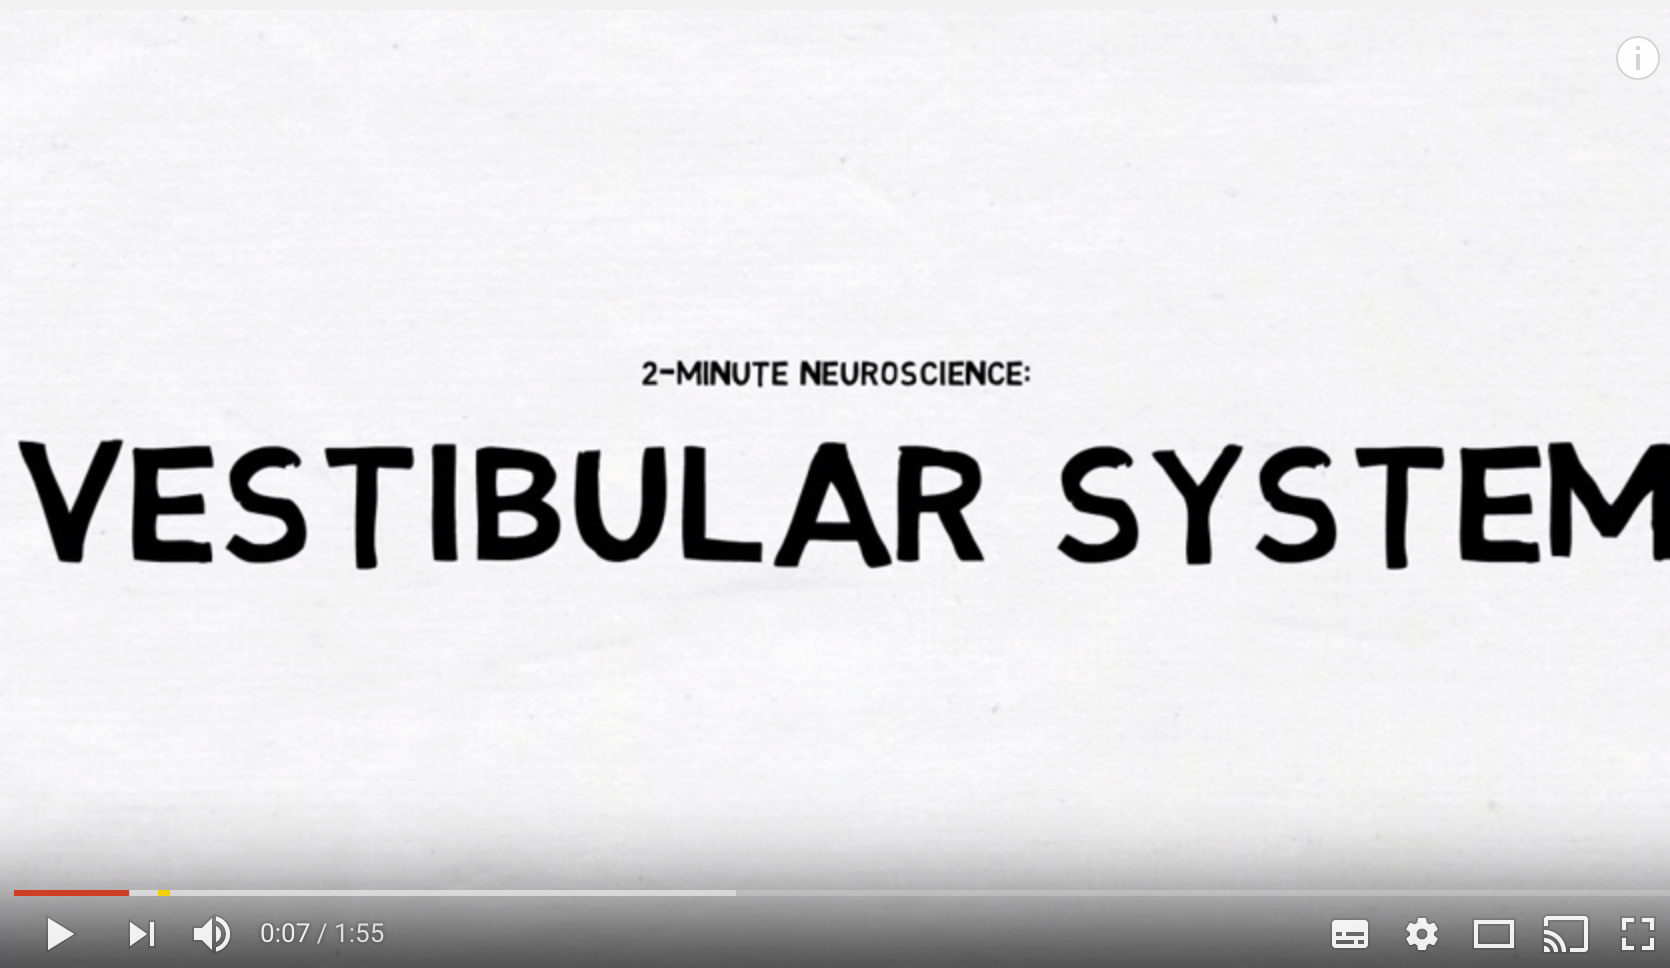
\includegraphics[scale=.3]{assets/vestibular} }
	\end{center}
\end{frame}

\begin{frame}
	Visually induced motion sickness (VIMS) is a specific type of motion sickness caused by a conflict between vision and both the proprioception and vestibular systems.  \\~\\
	
	According to Forbes, when a player is cycling a bike in VR, they have a tendency to lean to accommodate for corning, and as a consequence they fall off. \\~\\
	
	When tradition big screens cause VIMS the viewer can just look away but in VR this is not possible. 

\end{frame}




\begin{frame}
	\frametitle{Presence (again)}
	
	`Presence is the psychological state of subjective perception in which even though part or all of an individual's current experience is generated by and/or filtered through human-made technology, part or all of the individual's perception fails to accurately acknowledge the role of the technology in the experience.' \\~\\
	
	International Society for Presence Research, 2000
	\\~\\
	\href{http://ispr.info}{[ISPR Website]}	
	
\end{frame}


\begin{frame}
	``We see things not as they are, but as we are - that is, we see the world not as it is, but as moulded by the individual peculiarities of our mind'' \\~\\ - Philosopher, G.T.W Patrick. (1890) \\~\\
	\pause
	Reality is malleable. \\~\\ 
	\pause
	Our point of view is inseparable from our understanding of reality. 	
	
\end{frame}

\begin{frame}
	\begin{figure}
		\href{https://www.youtube.com/watch?v=zTrgHXNAs24}{ 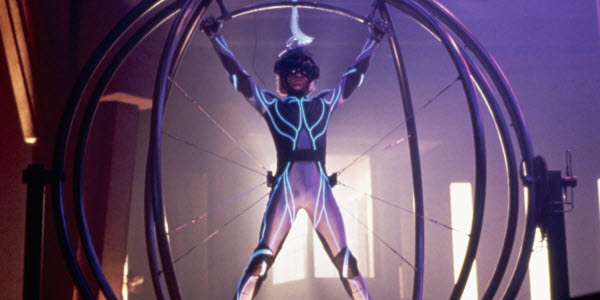
\includegraphics[scale=.3]{assets/mower}  }
		\caption{The Lawn Mower Man - 1992}
	\end{figure}
\end{frame}

\begin{frame}
	\frametitle{Duck Test}
	``a colloquial name for a method of testing if an experiencer has reached a state of presence, by monitoring their behaviour when threatened by a virtual object'' \\~\\
	- \href{http://www.vrglossary.org/glossary/duck-test/}{VRGlossary.org} \\~\\
	This could have an adverse effect if the experiencer realises that there is no actual risk - Presence is then broken.
		
\end{frame}

\begin{frame}
	\begin{figure}
		\href{https://www.youtube.com/watch?v=qD3w3cAhEYU}{ 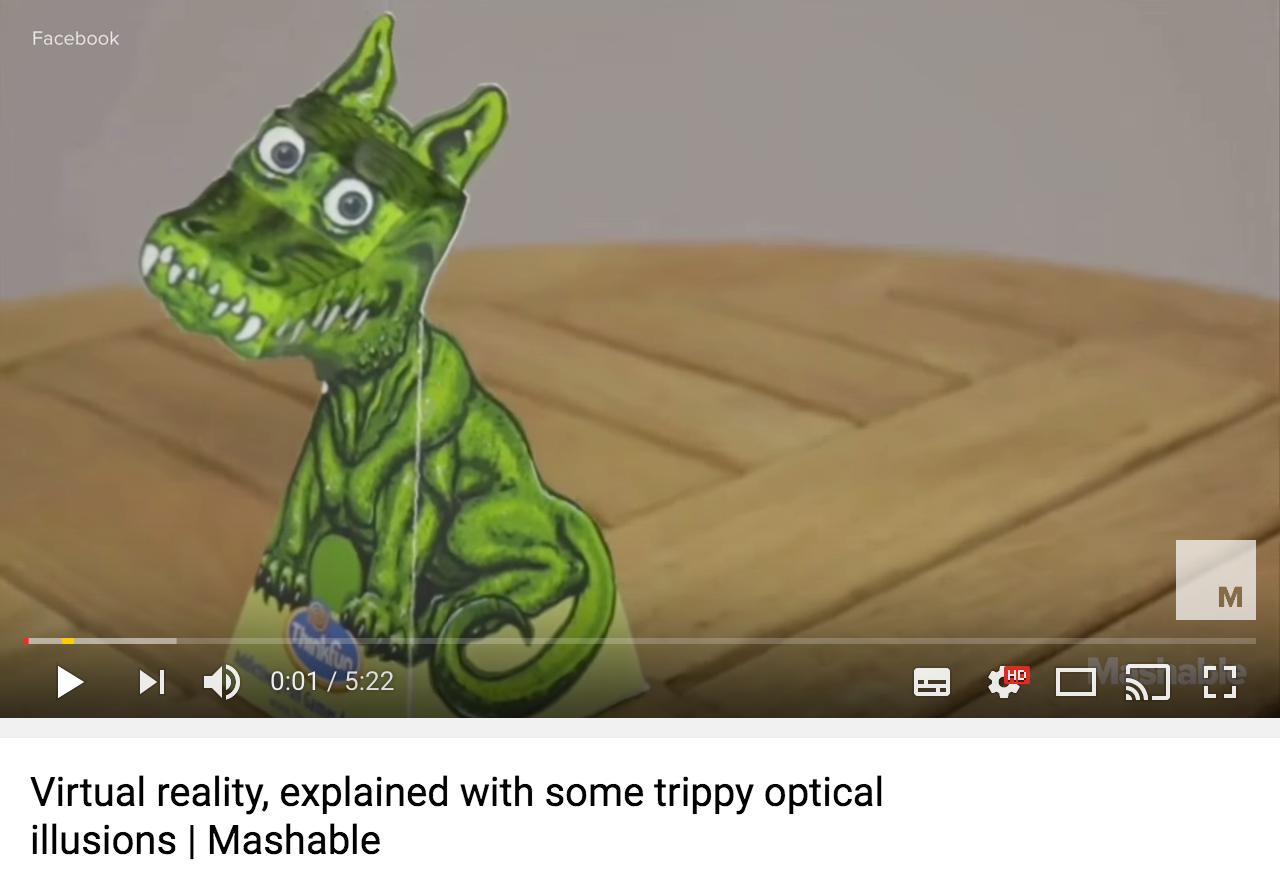
\includegraphics[scale=.4]{assets/optical}  }
		\caption{Michael Abrash, the chief scientist for Facebook's Oculus}
	\end{figure}
\end{frame}


\begin{frame}
	\frametitle{Types of Illusion}
	\begin{itemize}
		\item Boundary Completion
		\item Blind Spot \href{http://snowbrains.com/wp-content/uploads/2013/07/eyeball.jpg}{ (link to eye)}
		\item Depth Illusions - \href{https://www.youtube.com/watch?v=QmMTwjUdqbg}{Trompe-l'\oe il}
		\item Afterimage
		\item Motion Illusions - Watch these in VR as they cause motion sickness. 
	\end{itemize}
\end{frame}

\begin{frame}
	\frametitle{Illusions}
	V/AR are illusion based experiences \\~\\ 
	
	There are four main components to this illusion:
	\begin{itemize}
		\item the stable spacial place,
		\item self-embodiment,
		\item physical interaction \&,
		\item social communication.
	\end{itemize}
\end{frame}


\begin{frame}
	\frametitle{Reality is Subjective}
	By this point we are starting to get a sense that what we perceive is not necessarily real. \\~\\ \pause
	So what is getting in the way of reality? 
\end{frame}

%scan image from VR book p75
\begin{frame}
	\frametitle{Iterative Processing}
	\begin{figure}
		 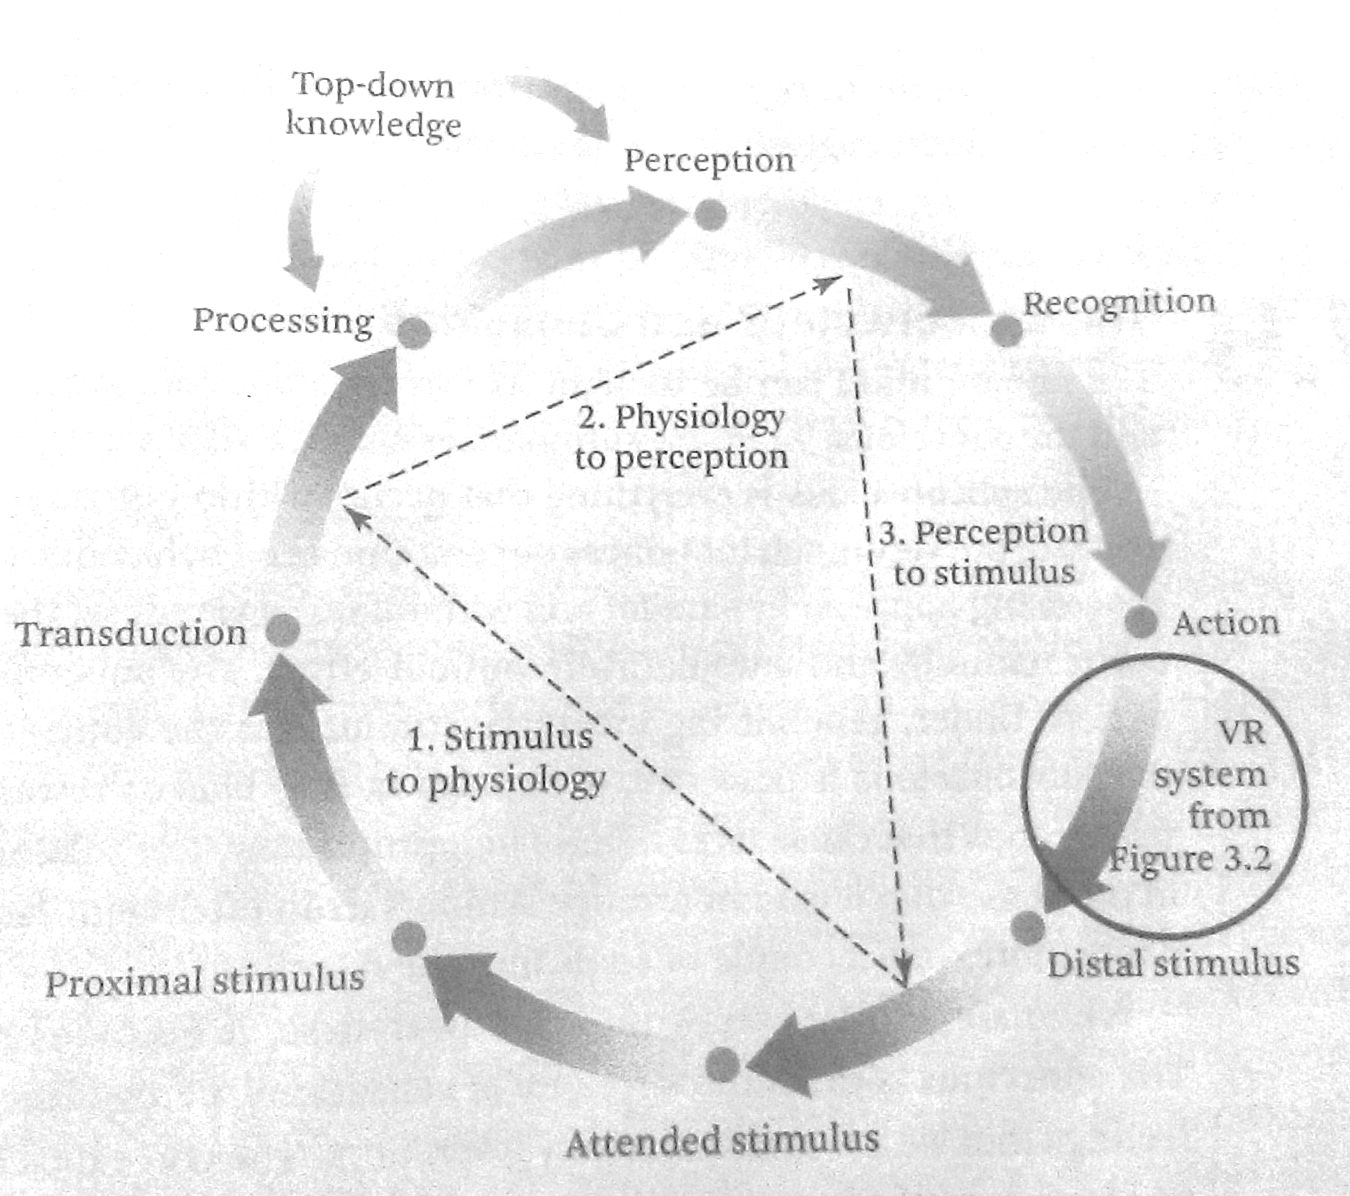
\includegraphics[scale=.1]{assets/iterative}
		 \caption{ We continually receive, process and perceive stimuli in an iterative loop}
		 
	\end{figure}
\end{frame}

\begin{frame}
	\frametitle{The Uncanny Valley}
	\begin{figure}
		 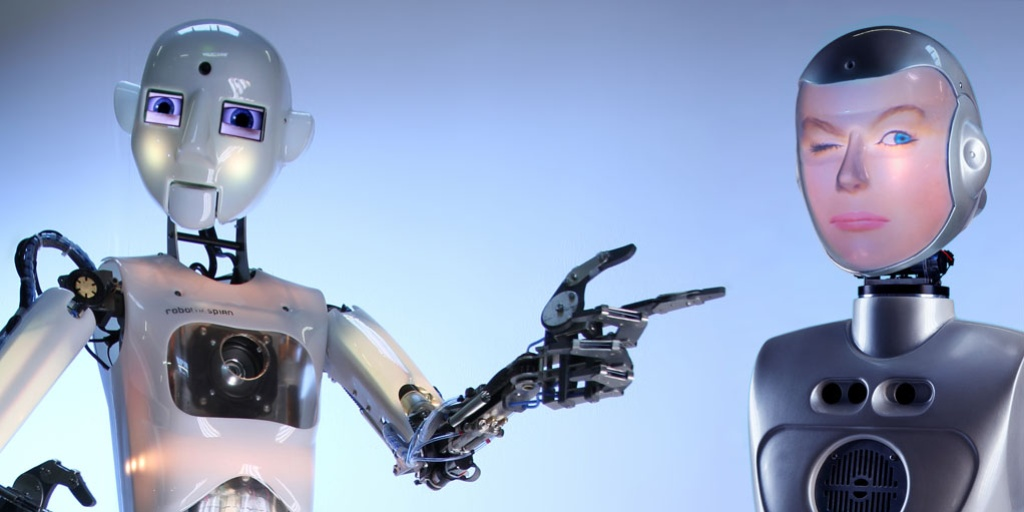
\includegraphics[scale=.3]{assets/bots}  
		 \caption{Engineered Arts - Penryn}
	\end{figure}
\end{frame}

\begin{frame}
	\begin{figure}
		 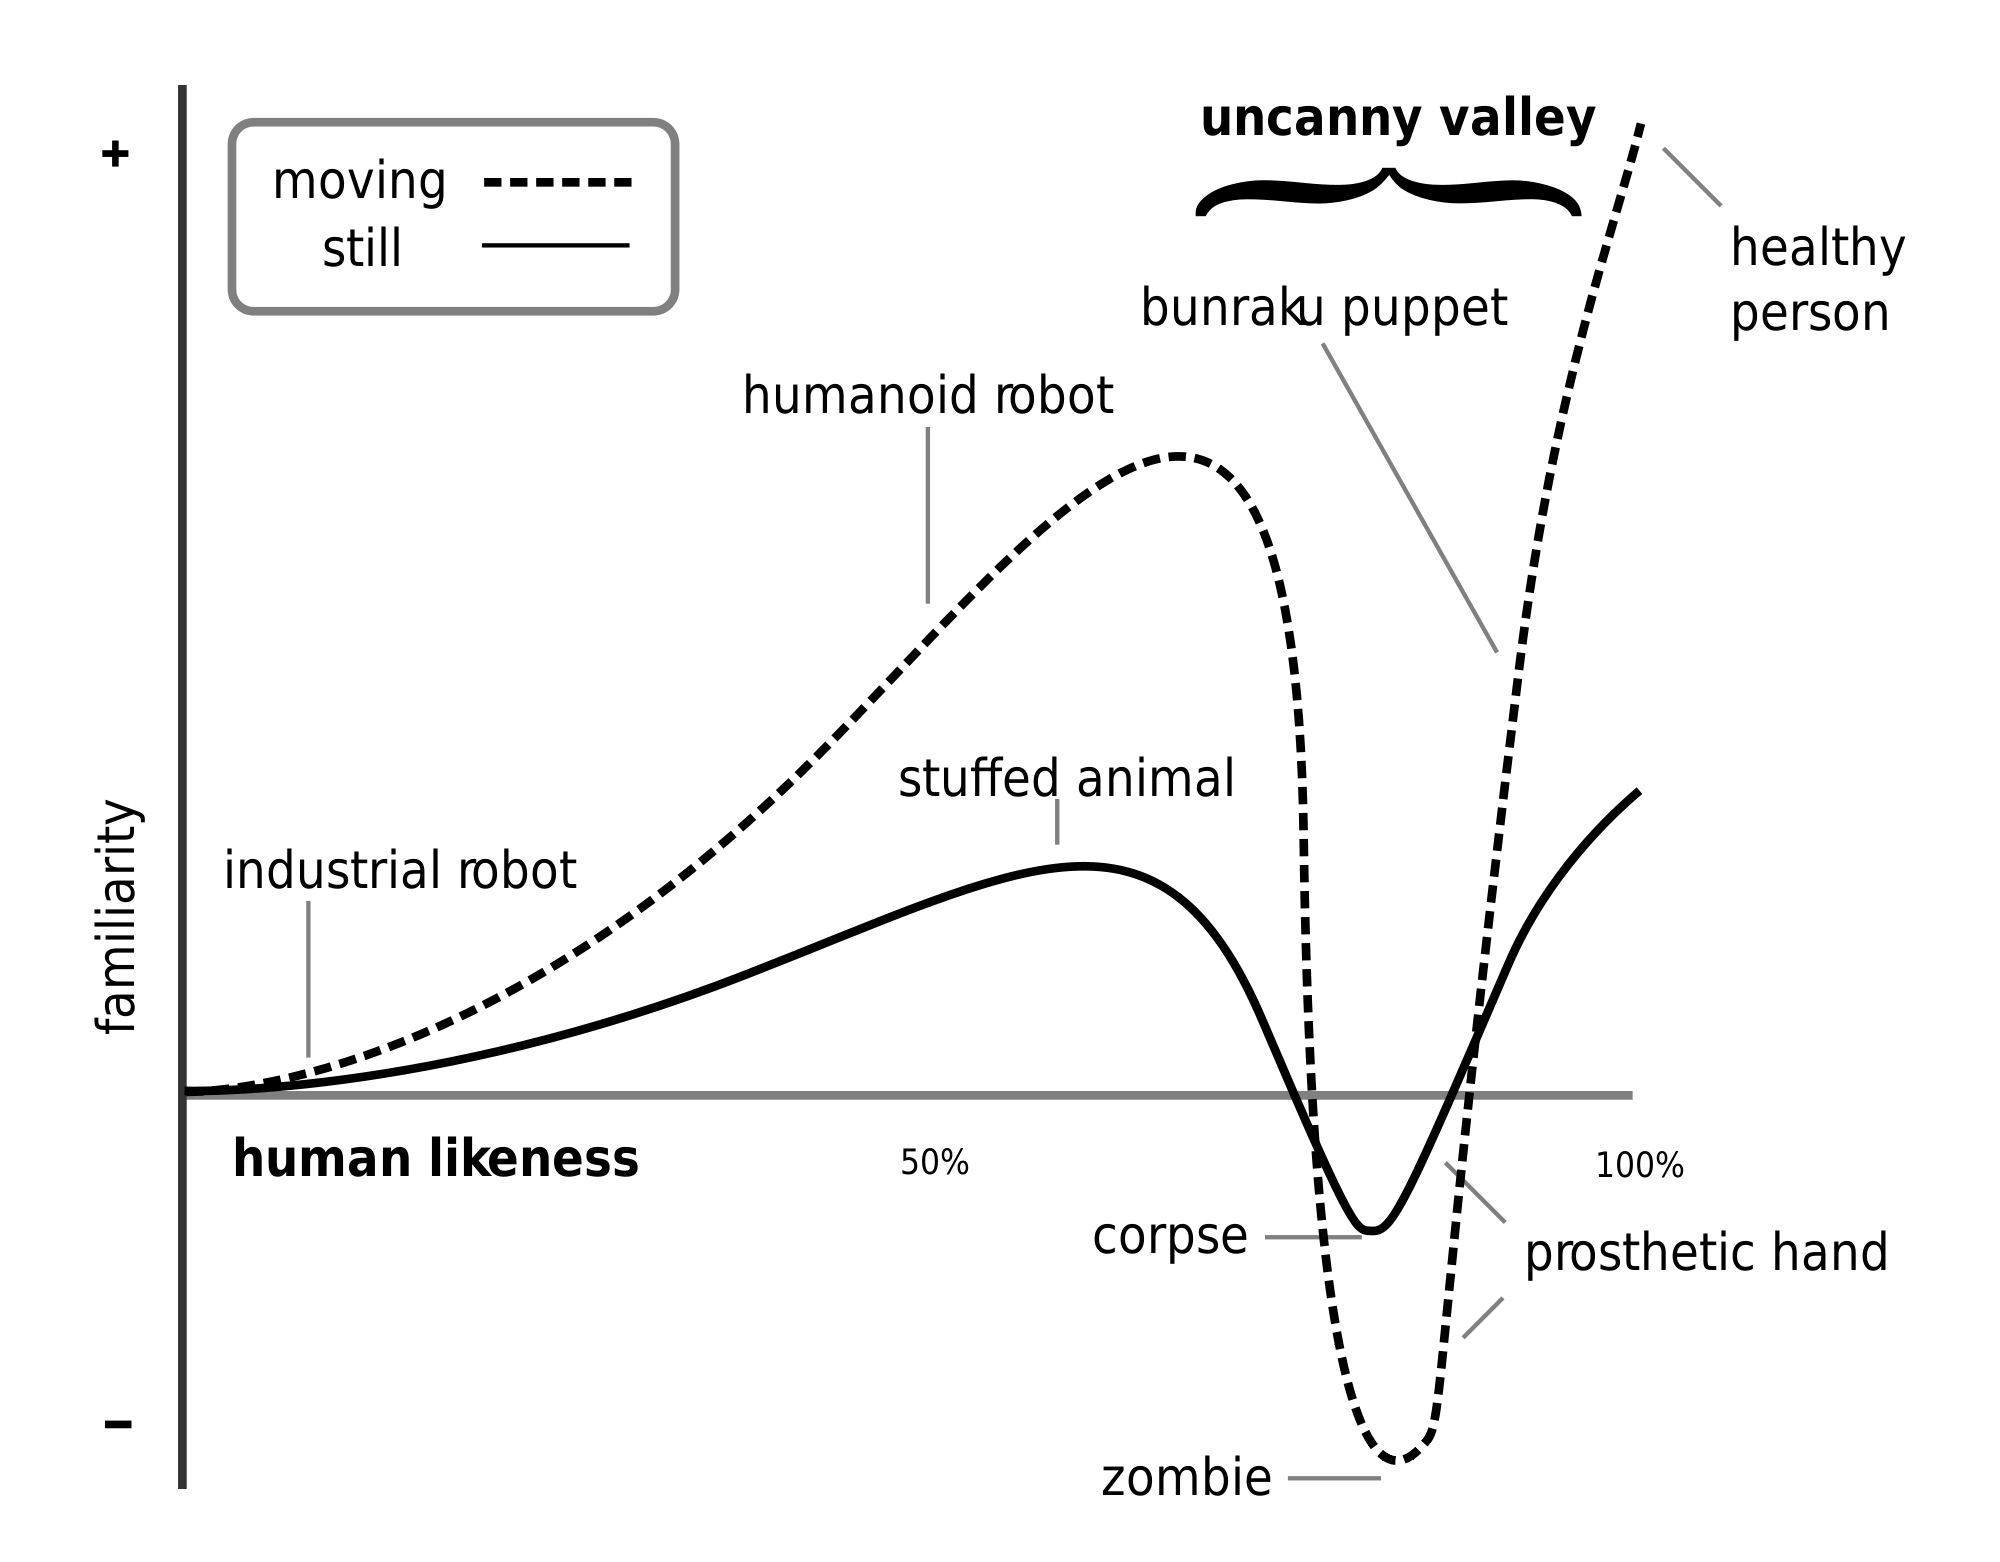
\includegraphics[scale=.13]{assets/uncanny}  
		  \caption{Masahiro Mori - }
	\end{figure}
\end{frame}

\begin{frame}
	\frametitle{Fidelity Continua}
	The notion of the uncanny valley applies to aspects of VR as well. These components have been defined as the Fidelity Continua. 
	
	\begin{itemize}
	 	\item	\textbf{Representation} fidelity - Hyper-realistic to abstract and non-objective worlds. 
		\item	\textbf{Interaction} Fidelity - Degree to which a interaction in VR corresponds with the same interaction in the real world.
		\item \textbf{Experiential} Fidelity - The degree to which the user experience matches the intentions of the VR creator. Procedural worlds have a very low experiential fidelity.
	 \end{itemize}
		
\end{frame}

\begin{frame}
	What do we want from V/AR? \\~\\
	Some aim to recreate reality to the highest fidelity. \\~\\
	Others seek to surpass it.
\end{frame}


\begin{frame}
	\frametitle{Misdirection}
	``That which directs a spectator away from the method and towards the effect'' \\~\\
	Curtis Hickman - Magician \& founder of THE VOID. \\~\\
	TRUTH/REALITY \textgreater  GUIDED PERCEPTION \textgreater  LIE/FANTASY \\~\\
	\href{https://www.youtube.com/watch?v=Ebwtq1HZJ2A}{LINK}
\end{frame}


\begin{frame}
	\frametitle{Sensation vs. Perception}	
	\begin{figure}
		\href{https://youtu.be/Ebwtq1HZJ2A?t=1051}{ 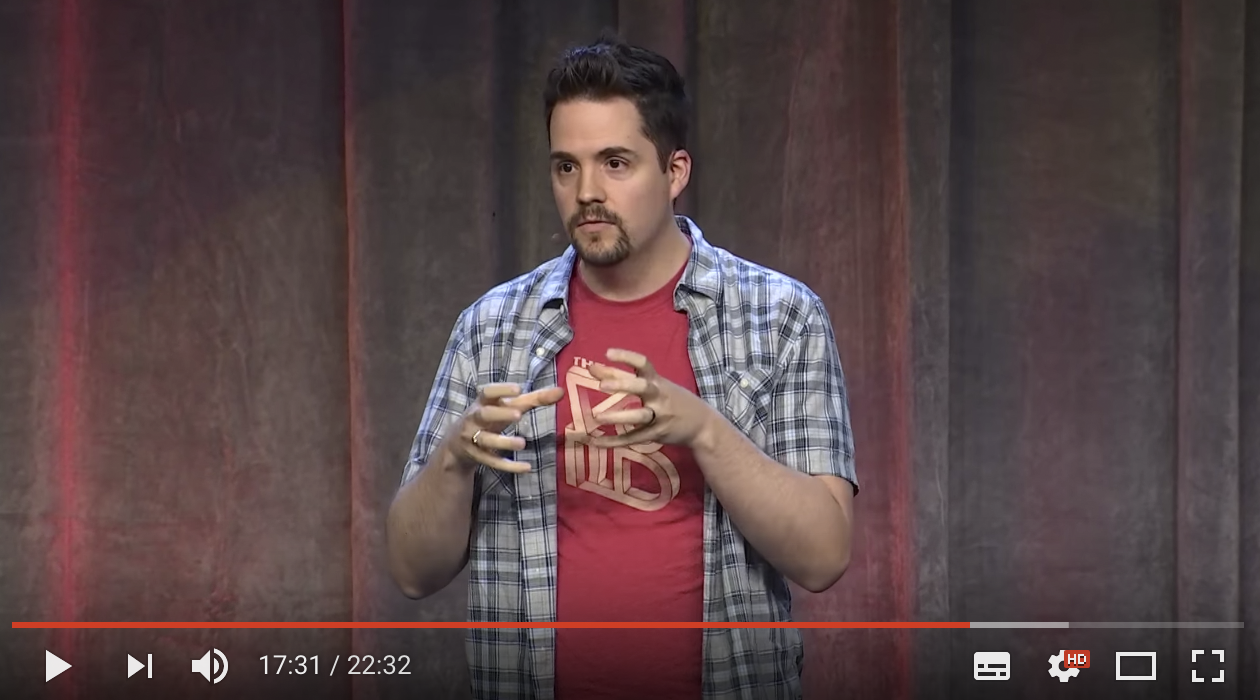
\includegraphics[scale=.17]{assets/sensation}  }
	\end{figure}
	\textbf{Sensation} - Lower level recognition of stimuli. \\~\\
	\textbf{Perception} - Higher level processing that combines information from the senses, filters it, organises it then interprets it to create \textbf{subjective}, conscious experience. 
\end{frame}


\end{document}








